\section{Introduction}
Satellite Internet is becoming important to commercial in-flight connectivity
(IFC). Travel measurements use repeated active tests to reveal latency, reachability, routing and transfer
behavior, but their interpretation requires known paths and observation limits.
Geostationary (GEO) and low Earth orbit (LEO) access have different architectures;
neither a low-latency reply nor a successful upload establishes aircraft movement,
access-link capacity or uninterrupted coverage.

Jang et al. compare GEO- and Starlink-based IFC using instrumented Android
devices across 25 flights~\cite{jang2025}. Their study motivates our long-term
goal: collect comparable network evidence across more routes through voluntary
participation on ordinary phones. Reproducing that study requires more than
replacing command-line tools with HTTP requests. Its routing and congestion
analyses depend on evidence that restricted mobile interfaces may not expose.
An unrooted application must therefore state which measurements it reproduces,
which quantities have different timing scopes, and which questions remain
unanswerable.

\system{} addresses three research questions. \textbf{RQ1:} What performance and
individual-probe evidence can the selected libraries collect without an
application-owned packet engine? \textbf{RQ2:} What collection and delivery
behavior can the prototype demonstrate under Android background operation?
\textbf{RQ3:} What additional validation is needed before interpreting its output
as a defensible IFC dataset? Comparing satellite operators remains a subsequent
campaign.

The prototype contributes a participant application, owned local evidence and a
private research workspace. It retains individual outcomes, original responses,
schedules and failures. Its evaluation distinguishes integration from accuracy,
collection from delivery, and endpoint rates from capacity: healthy-looking
probe results coexist with substantial unreceived evidence.

\section{Background and Related Work}
AmiGo uses travelers carrying instrumented Android phones as mobile vantage
points~\cite{varvello2023}. Its rooted devices and Termux environment support
researcher-controlled tools and detailed instrumentation. The IFC campaign of
Jang et al. applies this approach to satellite access~\cite{jang2025}. Our
objective is lower participant setup cost while preserving enough evidence to
support meaningful comparisons. We do not claim parity with its DNS/CDN,
same-socket congestion-control or flight-trajectory analyses.

Mobilyzer demonstrates controllable measurements through an Android library,
including resource management and measurement isolation~\cite{nikravesh2015}.
MONROE-Nettest shows that speed measurements depend on factors such as duration,
parallel flows and server placement~\cite{midoglu2018}. These designs motivate
our separation of serialized probe work from control observations and our
explicit recording of endpoint and method. SkyMeasure currently offers a narrower
local scheduling policy, rather than either platform's distributed experimental
control.

Prior Starlink studies provide complementary measurement perspectives.
Kassem et al. investigate connectivity from browsers and controlled
nodes~\cite{kassem2022}; Mohan et al. combine multiple sources and controlled
measurements~\cite{mohan2024}. Raman et al. identify satellite-provider
measurements in public datasets and complement them with recruited
testers~\cite{raman2023}. These studies support combining perspectives rather
than treating one endpoint's rate as a complete network characterization.

Izhikevich et al. reduce dependence on personally deployed satellite terminals
through remotely observable devices~\cite{izhikevich2024}. Their vantage points
and inferences differ from passenger-side collection. SkyMeasure instead targets
the phone's selected Wi-Fi connection. This positioning does not itself validate
either provider attribution or an airborne context. Our current ground results
establish software behavior only; reference measurements and genuine flights
remain necessary.

\section{System Design}
\subsection{Participant, service and researcher boundaries}
Figure~\ref{fig:architecture} summarizes the implemented data path. The phone
uses React Native and TypeScript, React Navigation and React Native Paper.
Participants accept research and M-Lab publication disclosures, enter flight
number, departure, arrival and expected duration, then select Start trip. These
are mandatory participant reports, not verified booking information. Expected
duration affects transfer spacing, never the ending time.

There is no visible participant login. Supabase anonymous authentication supplies
a pseudonymous identity; existing identities retain record ownership. Keychain
stores credentials, and previously enrolled devices can arm monitoring offline.
Missing credentials are not silently replaced. Researchers use Google sign-in
and explicit server roles. The backend derives ownership from verified tokens,
not request-supplied user identifiers. Identity reset cannot adopt another
identity's pending records.

OP-SQLite persists trips, measurements, events, context and retry state before
upload. Isolated FastAPI and UDP services run on a shared laboratory host;
Supabase PostgreSQL stores indexed research fields with original JSONB. A
Next.js dashboard on Vercel provides filters, grouped segments, timing views,
raw evidence and downloads. The laboratory host's physical region is unconfirmed.
It must not be assigned a convenient geographic label in the dataset.

\begin{figure*}[t]
\centering
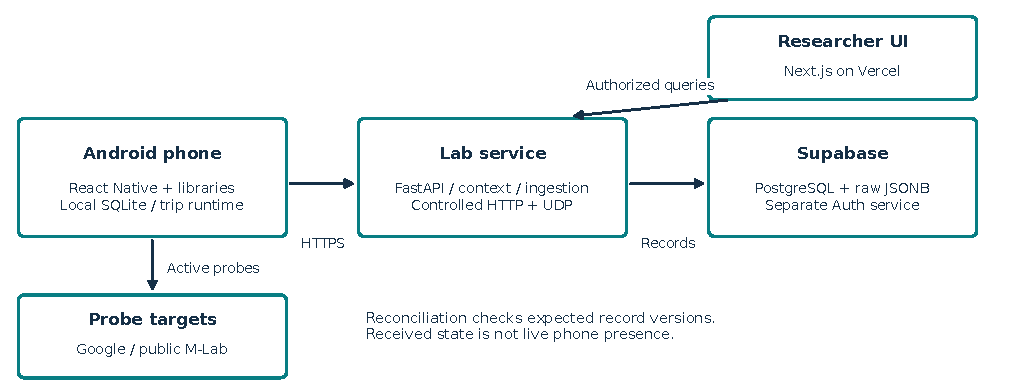
\includegraphics[width=.97\textwidth]{architecture.pdf}
\caption{Implemented logical architecture. The phone probes independent targets;
stored evidence passes through the laboratory API. Authentication has a separate
role. This is not a packet-level topology.}
\label{fig:architecture}
\end{figure*}

\subsection{ASN qualification and lifecycle}
The current detector, \code{asn-only-v1}, binds eligible work to selected Wi-Fi
using Android network APIs~\cite{androidbinding}. The context endpoint observes
the request's public address through configured trusted-proxy handling and
queries a local MaxMind GeoLite2-ASN database~\cite{maxmind}. Network identity
normally refreshes every minute, expires after two minutes, and is invalidated
when the Wi-Fi handle changes. Control evaluates nominally every 30 seconds;
two fresh matching evaluations at least 30 seconds apart admit collection.

The production registry contains six configured providers. The private pilot
additionally accepts AS12 and AS5384 through build/configuration gates. Any
test-ASN observation permanently marks the trip as ground-test evidence, which
research summaries exclude by default. An ASN covers a provider network, not
one router, and provider matching is not flight detection ground truth.
Automatic trips do not obtain GPS fixes; SSID is optional context only.

The lifecycle separates watching, collecting, paused and finished states.
Unknown identity on previously qualified, unchanged Wi-Fi retains outage probe
attempts. A fresh nonmatch pauses collection; changed Wi-Fi requires
requalification. The ten-minute loss-of-qualifying-connectivity grace begins
only after initial qualification. Stop, battery at or below 15\% while not
charging, and a 24-hour safety ceiling also end collection. Reported ending
reasons are operational inferences, not verified landings.

\section{Measurements and Scheduling}
\subsection{Library evidence and timing scope}
The Android ICMP and traceroute paths reuse pinned \code{icmpenguin}
1.0.0-rc.3 through thin adapters. ICMP requests contain 64 payload bytes plus
the eight-byte ICMP header. Returned bytes support header decoding and
sequence/payload correlation. The interface does not expose a verified reply
source address or permit matching the kernel-assigned request identifier.
Ten sequential attempts form a burst, with a 250-ms pause between attempts.
Nonresponse is retained even when the parent burst succeeds.

Traceroute uses UDP probes with increasing TTL, up to twenty hops and three
probes per hop. It preserves partial routes and library responses. Specialized
error classes do not always retain the original ICMP type/code; a
\code{host\_unreachable} label cannot be promoted to a verified wire-level
classification. This limitation matters even when the library reports arrival
at the destination.

TCP uses \code{react-native-tcp-socket}. Its duration extends from invocation to
the connection callback, including applicable resolution and bridge overhead;
it is not SYN-only or kernel-smoothed RTT. UDP uses \code{react-native-udp} and
a controlled echo service. Each burst sends twenty correlated 128-byte
datagrams, paced approximately 250 ms apart without waiting for each reply,
then allows a bounded reply grace. Payload matching, duplicates and reordering
remain observable; callback timing is not a kernel receive timestamp.

Controlled transfers request 5,000,000 download bytes and 1,000,000 upload bytes.
RNFS streams downloads to a file; React Native fetch uploads to an acknowledged
endpoint. Rates include the complete transaction's elapsed time. Available
partial file bytes survive a failed download, whereas an unacknowledged upload
may have unknown transferred bytes. Two consecutive failures disable that
controlled direction for the trip. HTTP RTT and loaded-latency code exist, but
loaded-latency tests are off in automatic trips.

One M-Lab NDT7 pair runs after a persisted randomized one-to-three-minute delay.
NDT7 is time-based, normally approximately ten seconds per direction, rather
than fixed-size~\cite{ndt7}. The pinned Android client has substantial owned
lifecycle, cancellation, accounting and routing changes. It is a maintained
source fork, not an unmodified SDK. Download uses client-received binary bytes;
upload prefers server receiver counters. Where only server TCPInfo is present,
the rate includes TLS/WebSocket overhead and is labelled accordingly. Current
private-pilot byte cutoffs are disabled; normal duration, watchdog, cancellation
and frequency safeguards remain.

\subsection{Statistics, deadlines and budgets}
For usable reply durations $r_i$, the primary burst statistic is the median;
the nearest-rank 95th percentile selects sorted rank $\lceil0.95n\rceil$.
Successive difference averages $|r_{i+1}-r_i|$ only over consecutive sequences
with both replies. It is not interchangeable with standard deviation or a
different protocol's jitter estimator. Complete-burst nonresponse is
$100(N-R)/N$. Incomplete bursts retain their counts without implying a complete
loss experiment. Transfer rates use $8B/(10^6t)$ Mbps with explicitly identified
bytes and elapsed seconds. Null means unavailable or inapplicable; zero remains
a valid observation.

Control and measurement work occupy separate asynchronous lanes on the same
JavaScript runtime. Probes remain serial. ICMP, UDP and TCP have minute deadlines
with initial offsets of approximately one, ten and twenty seconds; traceroute
starts after a minute and repeats every fifteen minutes. Deadlines advance from
the previous schedule. Late slots are skipped rather than replayed in a burst.
A control wake-up more than 90 seconds late records an unobserved collector gap.
Scheduled, invocation, callback and persistence times remain distinct. Android
elapsed-real-time observations help flag clock-discontinuous timings, but do
not make every library timestamp monotonic~\cite{androidclock}.

The first controlled pair is planned five minutes after qualification. Subsequent
spacing is $\max(5\text{ minutes},H/10)$ for reported expected duration $H$, with
at most ten pair reservations. Heavy jobs are spaced apart. Per-trip allocations
are 60 MiB controlled transfers, 20 MiB diagnostics/context and 20 MiB live
uploads. They never reset at segment boundaries. M-Lab is outside those limits
in the current private build. These are application reservations, not interface
or carrier counters; retransmissions, transport overhead and post-trip sync are
additional.

\subsection{Why retain libraries rather than our earlier packet engine?}
An earlier branch maintained C++ probes, Linux error-queue metadata and
short-connection TCPInfo snapshots. Reusing libraries reduces owned measurement
code but relinquishes verified error provenance and handset kernel statistics.
These are limits of the selected interfaces, not every unrooted approach.
Android adapters still select networks, cancel operations and serialize results;
React Native alone does not provide those functions. Pinned dependencies require
maintenance review. Neither branch measures congestion-window evolution on the
controlled-transfer socket. Restoring native telemetry should answer a research
requirement rather than enlarge a CSV schema.

\section{Durability, Uploads and Interpretation}
Every fifteen minutes the runtime closes a segment, cancelling outstanding work
if necessary, and attempts synchronization for nominally 25 seconds. The detector
and foreground-service lifecycle remain armed. Qualification, deadlines and
cumulative reservations survive rotation. The next segment records the actual
upload pause, which is a sampling gap rather than inferred network downtime.

The server registers each closed segment's immutable expected record IDs and
versions before accepting batches. Requests contain at most fifty records and
target 512 KiB of serialized JSON; an individual large record remains intact.
Local acknowledgements are durable. Completion requires every expected version,
not merely a successful HTTP response. Interrupted requests may commit remotely
before the phone receives their acknowledgements, so retries must be idempotent.
Trip revisions are monotonic and a closed trip declares its final segment count.

Post-trip synchronization uses owner-scoped, persisted round-robin opportunities
across pending trips and historical standalone sessions. This prevents one old
backlog from monopolizing later opportunities. Retry backoff and Wi-Fi preference
still apply. The current Retry uploads button opens one bounded opportunity; it
does not force backoff expiry or drain all evidence continuously. Background-fetch
provides opportunistic Android retries, not guaranteed execution after force-stop.

Measurements, individual samples, repeated context and events have different
granularities. The combined CSV repeats parent/context fields for sample rows
and retains parents without samples. Dashboard totals group unique parents;
they must not sum repeated parent bytes or values. Original JSON remains the
authoritative evidence. Neither an active-looking trip card nor a received
segment proves the phone is currently collecting.

\section{Ground Evaluation}
\subsection{Evidence and completed integration checks}
The evaluation freezes a read-only server snapshot on 16 November and retains
unchanged private inputs with SHA-256 provenance. All new experiments are ground
tests. A historical ten-minute library experiment produced 41 parent measurements,
98/100 ICMP replies, 40/40 UDP replies and 10/10 TCP connections. Its HTTP
transfers traversed USB forwarding, so their rates are not Internet-capacity
results~\cite{artifact}. The preserved custom-engine baseline also had different
methods and conditions; it cannot establish comparative reliability.

A 15 November short trip ran approximately twenty minutes and closed two
segments. All 435 expected records reconciled, and stopped-phone inspection
confirmed all 327 and 108 queue entries acknowledged. Its 64 measurements
included 170/170 ICMP replies, 352/360 UDP replies, 19/19 TCP connections and two
reported successful traces. Three controlled downloads and two of three uploads
succeeded. The screen was locked through rotation with USB attached; that test
does not establish unplugged endurance.

Dated checks report 288 mobile, 49 backend, eighteen browser and seven native
NDT7 tests; one optional PostgreSQL check was skipped locally. These software
checks do not establish network accuracy. Pilot 1.2.2 is the tested artifact;
not every export identifies its full application build.

\subsection{Received portion of the newest long trip}
At the snapshot, the newest trip declared 58 segments but supplied only nine
manifests: eight reconciled and one partial. The registered manifests expected
2,666 records; 2,625 were present, with 41 versions missing and no unexpected
versions. Forty-nine additional declared positions had no manifest, so their
record totals are unknown. Received intervals cover approximately the first
2.25 hours. The last trip update preceded the audit by approximately fourteen
hours and forty minutes. Its active state cannot establish current collection
or a completed run duration.

\begin{figure*}[t]
\centering
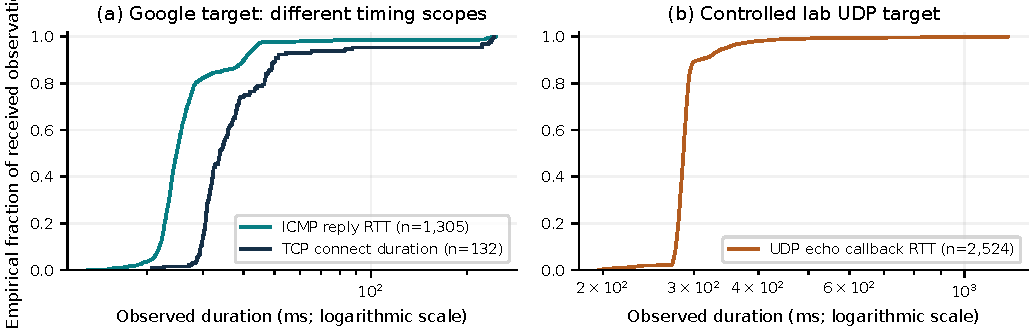
\includegraphics[width=.97\textwidth]{latency-cdf.pdf}
\caption{Measured distributions from the newest trip's received portion.
Nonresponses are excluded from these conditional CDFs but included in
Table~\ref{tab:results}. TCP invocation-to-callback duration is not ICMP RTT;
the controlled UDP destination also differs from Google. These curves do not
establish protocol superiority or reference accuracy.}
\label{fig:cdf}
\end{figure*}

\begin{table}[t]
\centering\small
\caption{Newest trip: received evidence only. Durations are pooled over valid
replies or connections, not averaged burst medians.}
\label{tab:results}
\begin{tabularx}{\columnwidth}{@{}lY r@{}}
\toprule
Method & Observed outcome & Median (ms)\\
\midrule
ICMP & 1,305/1,320 replies & 24.75\\
UDP & 2,524/2,640 replies & 286.51\\
TCP & 132/132 connected & 33.80\\
Traceroute & 9/9 reported arrival & --\\
Download & 1/3 completed & --\\
Upload & 2/4 completed & --\\
\bottomrule
\end{tabularx}
\end{table}

The received portion contains 414 parent measurements and four unsuccessful
controlled transfers (Table~\ref{tab:results}). All 132 ICMP bursts completed,
but fifteen individual attempts lacked replies; UDP had 116 nonresponses among
2,640 attempts. Figure~\ref{fig:cdf} retains the different targets and timing
scopes. UDP's greater median cannot be attributed to protocol overhead: Google
and the laboratory are different destinations. Nine traces reported arrival,
with 44 timeouts among 295 hop observations. Ambiguous library labels remain
qualified rather than converted into verified ICMP classifications.



The completed 5 MB controlled download took 59.40 seconds, approximately
0.67 Mbps. Two later downloads failed after observing 15,760 and 8,000 file
bytes. Headers arrived after approximately 11--15 seconds. Two uploads completed
at 0.75 and 0.52 Mbps; two timed out near thirty seconds. Each direction then
recorded its consecutive-failure cutoff. Missing later controlled transfers can
therefore be deliberate policy. These observations identify a server/path
investigation, not a measured satellite bottleneck.

The same trip's NDT7 pair completed at reported rates of 133.90 Mbps download
and 112.89 Mbps upload, with the latter using server TCP receiver counters.
Across three completed ground pairs, client payload totals were 251.4, 295.8
and 305.6 MiB (Figure~\ref{fig:mlab}). This sample does not establish a universal
data allowance. It does show that earlier caps could terminate otherwise useful
ground benchmarks. A proposed 200 MiB per direction remains a future policy,
not a limit applied to these runs or a guaranteed billed-data ceiling.

\begin{figure*}[t]
\centering
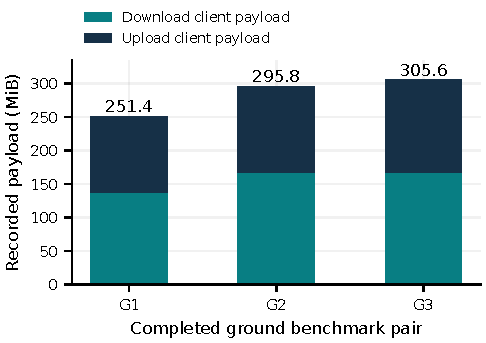
\includegraphics[width=.46\textwidth]{mlab-payload.pdf}\hfill
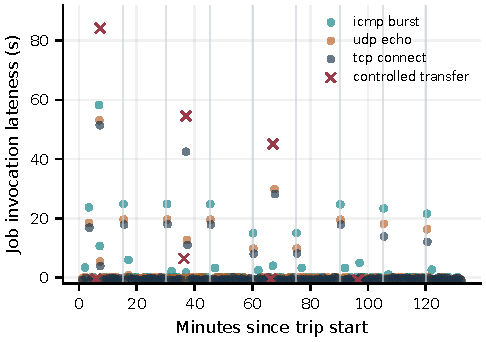
\includegraphics[width=.46\textwidth]{schedule-lateness.pdf}
\caption{Left: client payload for three completed 15 November ground benchmark
pairs; these are not carrier byte totals. G1 is the reconciled short trip; G3
is the newest long trip. Right: scheduled job invocation lateness in the received
slice, with grey upload-pause bands. Scheduled cadence does not establish
regular execution.}
\label{fig:mlab}
\label{fig:schedule}
\end{figure*}

\begin{figure*}[t]
\centering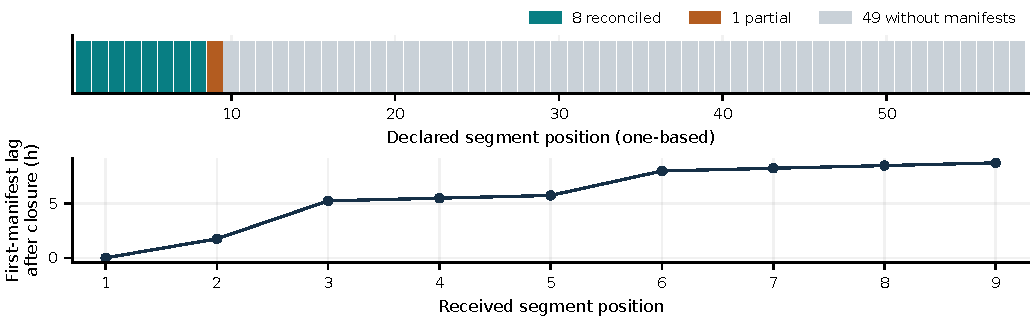
\includegraphics[width=.97\textwidth]{delivery.pdf}
\caption{Delivery at the frozen snapshot. Top: 58 declared positions, with
eight reconciled, one partial and 49 lacking manifests. Bottom: first manifest
receipt lag for the nine registered segments, measured from their recorded
closure. These are not completion times, and absent manifests do not prove
that local measurements were lost. Receipt differences use phone/server wall
clocks without independent clock calibration; they are not transport-latency
measurements.}
\label{fig:delivery}
\end{figure*}

\subsection{Scheduling and delivery findings}
In the received slice, maximum detector spacing was 40.04 seconds; eight
received health summaries reported no collector gaps. The largest recorded job
lateness was 84.22 seconds (Figure~\ref{fig:schedule}). Most observations were
background/screen-off; all 801 context snapshots reported not charging, and some
power observations reported device idle. These are recorded API states, not an
independent energy experiment or proof about missing later intervals.



Delivery is substantially behind collection reporting (Figure~\ref{fig:delivery}).
The latest manifest reserves 20,824,718 of 20,971,520 live-upload bytes, or
99.30\%, leaving 146,802 bytes for further requests and conservative response
reservations. Received upload events include four opportunity cancellations and
two request timeouts. Near-exhaustion can block request sizes and is a plausible
contributor, but the phone's unsent queue is needed to establish the final cause.
Removal of the M-Lab cutoff did not remove this separate allocation. Earlier
batch-query and starvation fixes enabled short-trip reconciliation; they did not
resolve this longer-run backlog.



Offline checks found no unexpected versions in received manifests. Their generic
timestamp validator flagged the epoch-millisecond trip start in all nine
envelopes because it expects ISO text. This is an identified analyzer mapping
gap, not nine malformed probe measurements. The other measurement checks found
no errors; 251 warnings qualify traceroute labels. Passing consistency checks
does not prove that the measured quantities match wire-level ground truth.

\section{Planned Independent Validation}
First, recover the pending phone evidence and reconcile every closed segment; do not erase
local storage to make a dashboard appear complete. A repeated one-hour,
unplugged, locked-screen run will compare ordinary battery settings with allowed
background access. Exact record reconciliation, visible interruptions and no
unexplained control spacing above two minutes are engineering acceptance
criteria, not claims already met by the full overnight dataset.

Second, a laptop on the same Wi-Fi will run matching ping payloads, UDP echoes,
TCP connections and UDP traceroutes against the same resolved destinations.
At least fifty twenty-packet UDP rounds provide 1,000 observations; one round
alone has five-percentage-point loss resolution. Independent NDT7 and controlled
HTTP transfers will run sequentially with phone transfers to limit contention.
Cross-device agreement is a sanity check, not same-device ground truth.

Third, a dedicated Linux gateway will capture the phone-facing traffic and apply
controlled impairment. Proposed added-RTT conditions include 0, 40, 150, 300 and
600 ms, with calibrated half-delay on each direction; loss and rate limits will
vary separately before combinations. Captures will check payload correlation,
sent/replied counts and actual impairment. App callback timing will be compared
with gateway packet timing using matched observations and clock scope, rather
than subtracting unrelated clocks. Planned plots include paired error/limits
of agreement, delay/loss response, scheduling-gap distributions and delivery
curves. No synthetic validation outcomes are presented as measured results.

Finally, consented real flights will evaluate provider attribution, captive
portals, transitions and policy cost across aircraft and phones. Flight labels
must have independent corroboration. ASN and Starlink PTR changes identify
provider/egress evidence; neither establishes a satellite handover. The validation
matrix and proposed plots appear in Appendix~\ref{app:validation}.

\section{Limitations, Ethics and Conclusion}
The main validity threats are shared ground conditions, a small benchmark sample,
different endpoints, callback/library timing, Android scheduling and incomplete
uploads. A missing server record is neither a failed probe nor zero traffic.
No matched Linux accuracy campaign or real-flight detection evaluation is
complete. Current libraries retain useful packet evidence but do not expose
full traffic capture, handset congestion-window evolution or satellite identity.
The custom engine's historical short-connection TCPInfo snapshots do not supply
same-socket congestion behavior during HTTP load.

Participation is pseudonymous, not anonymous in a strong privacy sense: network
identifiers, public addresses, time and reported flight information can be
identifying. No coordinates or raw location objects belong in persisted or
exported data. M-Lab public-data publication requires explicit disclosure.
Public recruitment remains contingent on approved participant text, appropriate
institutional review, enrollment protection and operational deletion procedures.
The paper releases de-identified plotting tables, not private raw records or
deployment credentials.

SkyMeasure demonstrates an operational unrooted pipeline. RQ1 yields useful,
bounded library evidence; RQ2 yields short-trip reconciliation and unresolved
long-run delivery. RQ3 remains the independent validation needed before a
defensible crowdsourced IFC campaign.
